Este capítulo dedica-se a explanar como a aplicação proposta para a intervenção ao problema, anteriormente descrito, executa suas ações e descreve o fluxo de ação entre atividades e interação com outras aplicações. Para isso, é mostrado os fluxos e atividades de suas ações em figuras e descrito detalhadamente o que pode ser extraído das imagens.

\section{Diagrama de Atividades}
O intuito da utilização do Diagrama de Atividades é dar ênfase ao fluxo de controle na execução de um comportamento realizado por um sistema, mostrando o fluxo entre atividades em um sistemas. As atividades podem ser referidas como um fluxo sequencial ou ramificação de atividades que interagem entre si e outros objetos para realizar ou sofrer ações. Descrevendo assim, uma modelagens a função do sistema \cite{Booch:2012}.  

Ao iniciar aplicação é apresentada a tela inicial contendo um campo para entrada de dados para a pesquisa e botões de escolha. Este campo é utilizado para a entrada da sentença em linguagem natural para busca do usuário que esta utilizando a aplicação. Após a inserção da sentença, é necessário a escolha da próxima ação do usuário. A ação de pesquisar e a de limpara o campo da entrada.

Ao clicar no botão de limpar, é reapresentado a tela inicial contendo novamente os botões de escolha, juntamente com o campo para a entrada para a busca. Caso o botão de pesquisar for acionado, é iniciado o processo de busca dos dados solicitado ao usuário e retornado ao mesmo caso forem encontrados registros na base de dados onde-se encontra estes dados persistidos.

Todo este fluxo e atividades são desmostrado na \autoref{diagact} com o intuito de facilitar o esclarecimento e melhorar o entendimento a respeito da aplicação proposta.


\begin{figure}[!htb]
        \caption{\label{diagact}Diagrama de Atividade}
        \begin{center}
                \includegraphics[width=\textwidth]{imagens/diagact.eps}
        \end{center}
        \legend{Fonte: Autor}
\end{figure}

\newpage
\section{Fluxo de funcionamento da aplicação}
Esta sessão dedica-se a explanar mais detalhadamente todo o fluxo da aplicação proposta. Usando como base a \autoref{diagfluxo}, é descrito cada atividade contido no formato: - <Nome atividade>: Detalhamento.

\clearpage
\begin{itemize}
	\item Mostrar tela inicial - A aplicação renderiza tela inicial contendo o campo para entrada da busca e os botões de escolha Limpar e Pesquisar.
	\item Entrada de dados - É aguardado a entrada da sentença em linguagem natural solicitado pelo usuário.
	\item Selecionar opção - O usuário deve escolhe entre as opções Limpar campo e Pesquisar.
	\item Limpar - Caso o usuário escolha a opção Limpar, é limpada o campo e novamente é renderizado a tela inicial para entrada de nova busca.
	\item Pesquisar - Caso o usuário escolha a opção Pesquisar, a aplicação cria uma requisição HTTP do tipo Post contendo em seu corpo a sentença do usuário, para o endereço da API LUIS.
	\item Envia requisição ao LUIS - Após, o envio é realizado e a aplicação aguarda o retorno da solicitação.
	\item Recebe requisição - A API LUIS recebe a requisição e processa a sentença do usuário.
	\item Envia solicitação traduzida no formato JSON - Após o processamento, a API responde a solicitação traduzindo as entidades e intenções identificadas na sentença.
	\item Recebe tradução - Recebe a tradução da sentença no formato JSON.
	\item Confirma dados recebidos - A aplicação solicita confirmação das intenção e os atores indentificado pelo LUIS estão corretas.
	\item Mostrar opções Continuar e Refazer - Para confirmação, o usuário deve escolher as opções Continuar ou Refazer para dar continuidade no fluxo.
	\item Refazer - Caso escolha Refazer, é novamente mostrada a tela inicial dando a possibilidade que o usuário refaça a sentença, para posteriormente refazer novamente tradução.
	\item Continuar - Se a opção continuar for escolhida, a aplicação dará continuidade ao fluxo para busca dos dados.
	\item Envia requisição ao Elasticsearch - Posteriormente, a aplicação encaminha a requisição  de busca dos dados na base da API Elasticsearch e aguarda o retorno da requisição.
	\item Recebe requisição - A API Elasticsearch recebe a requisição da aplicação e realiza o a procura pelos dados solicitados e retorna uma resposta caso os dados são encontrados ou não.
	\item Recebe a resposta - A aplicação recebe a resposta contendo os dados ou não no formato JSON.
	\item Mostra resposta ao usuário - Aplicação mostra os dados ao usuário e questiona se deseja fazer uma nova busca.
	\item Mostra opção Sim/Não - É mostrada as opções Sim e Não em forma de botões interativos o qual o usuário pode escolher continuar a realizar buscas por dados ou finalizar aplicação.
	\item Sim - Caso opção Sim for escolhida, a aplicação mostra a tela inicial possibilitando ao usuário realizar novas buscas.
	\item Não - Caso a opção escolhida for Não, a aplicação é encerrada.
\end{itemize}


\begin{figure}[!htb]
        \caption{\label{diagfluxo}Fluxo de funcionamento da aplicação}
        \begin{center}
                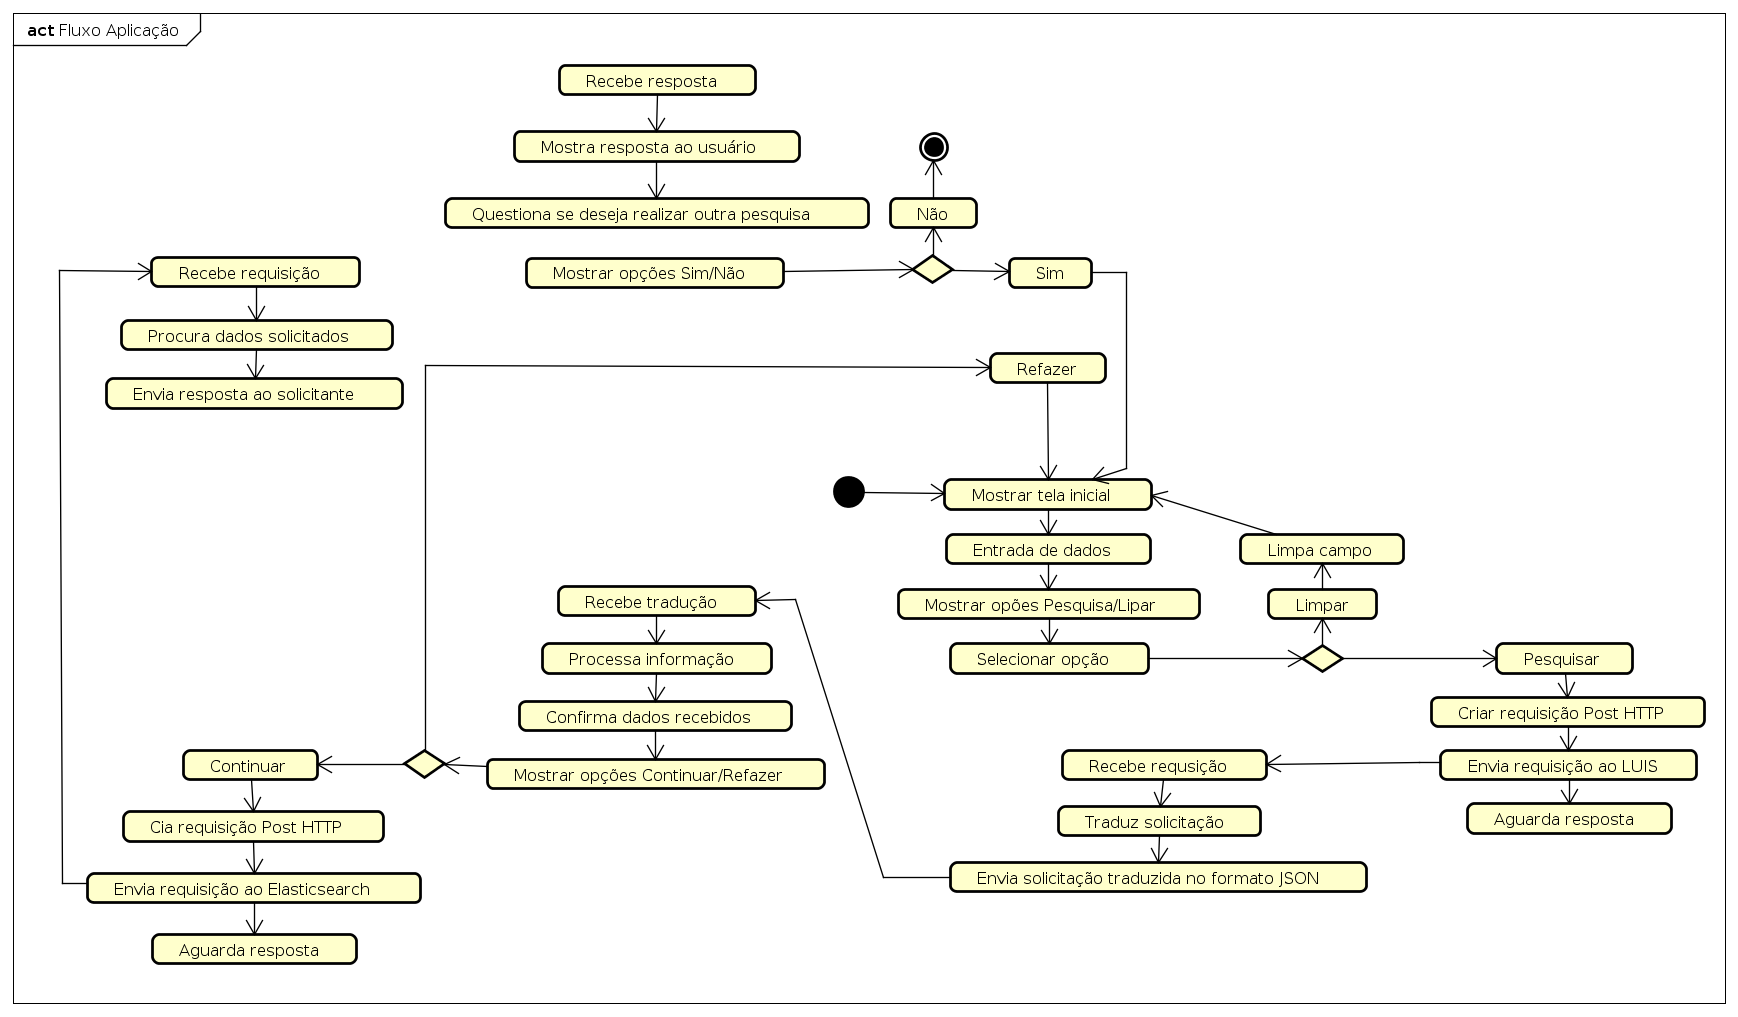
\includegraphics[angle=90, width=\textwidth, height=\textheight]{imagens/diagfluxo.eps}
        \end{center}
        \legend{Fonte: Autor}
\end{figure}
